\documentclass[a4paper]{report}

%====================== PACKAGES ======================

%\usepackage[french]{babel}
%\addto\captionsfrench{\renewcommand{\tablename}{Tableau}}  % Localization
\usepackage[utf8]{inputenc}
%pour gérer les positionnement d'images
\usepackage{float}
\usepackage{eurosym}
\usepackage{amsmath}
\usepackage{empheq}
\usepackage{graphicx}
\usepackage[colorinlistoftodos]{todonotes}
\usepackage{url}
%pour les informations sur un document compilé en PDF et les liens externes / internes
\usepackage{hyperref}
%pour la mise en page des tableaux
\usepackage{array}
\usepackage{tabularx}
%pour utiliser \floatbarrier
%\usepackage{placeins}
%\usepackage{floatrow}
%espacement entre les lignes
\usepackage{setspace}
%modifier la mise en page de l'abstract
\usepackage{abstract}
%police et mise en page (marges) du document
\usepackage[T1]{fontenc}
\usepackage[top=1cm,bottom=2cm,left=2cm,right=2cm]{geometry}
%Pour les galerie d'images
%\usepackage{subfig}
\usepackage{graphicx}
\usepackage{fancyhdr}
\usepackage{subcaption}
\usepackage{textcomp}  % for euro symbol e
\usepackage[table]{xcolor}
\usepackage{colortbl}
\usepackage{booktabs}
\usepackage{siunitx}
\usepackage{makecell}
\usepackage{multirow}
\usepackage{hhline}
\usepackage{abstract}
\usepackage{textcomp} % pour le symbole €
\usepackage{siunitx}
\usepackage{verbatim}
\usepackage{fancyvrb}
\usepackage{listings}
\usepackage[most]{tcolorbox}
\tcbuselibrary{listings,breakable}

\newtcolorbox{examplebox}{
  colback=gray!5,
  colframe=gray!50,
  boxrule=0.5pt,
  arc=2mm,
  breakable
}

\newtcblisting{pythonbox}{
  listing only,
  listing engine=listings,
  listing options={
    language=Python,
    basicstyle=\ttfamily\small,
    numbers=left,
    breaklines=true,
    showstringspaces=false,
    columns=fullflexible
  },
  colback=gray!5,
  colframe=gray!50,
  boxrule=0.5pt,
  arc=2mm,
  left=1mm,
  right=1mm,
  top=1mm,
  bottom=1mm,
  breakable,
  
}

\newtcblisting{impbox}{
  listing only,
  listing engine=listings,
  listing options={
    basicstyle=\ttfamily\small,
    breaklines=true,
    showstringspaces=false,
    columns=fullflexible
  },
  colback=gray!5,
  colframe=gray!50,
  boxrule=0.5pt,
  arc=2mm,
  left=1mm,
  right=1mm,
  top=1mm,
  bottom=1mm,
  breakable,
  
}

\lstset{
  frame=single,
  basicstyle=\ttfamily\small,
  columns=fullflexible
}

\sisetup{
  detect-all,
  per-mode=symbol
}

 
% ---------- Helpers ----------
\newcolumntype{Y}{>{\centering\arraybackslash}X} % centered tabularx column 
 
% ---------- KPI colors ----------
\definecolor{kpigreen}{RGB}{140,255,140}
\definecolor{kpiyellow}{RGB}{255,245,170}
\definecolor{kpired}{RGB}{255,140,140}


% --- Logo + header sizing ---
\newlength{\logoht}
\setlength{\logoht}{2cm}

\setlength{\headheight}{1.5cm} % >= 2cm logo, avoids warnings (2.3cm ~ 65pt)
\setlength{\headsep}{12mm}      % optional: gap between header and text
\geometry{top=2.5cm,bottom=2cm,left=1.5cm,right=1.5cm}

\newcommand{\vcenterinhead}[1]{%
  \raisebox{0.5\dimexpr\headheight-\height\relax}{#1}%
}

\pagestyle{fancy}
\fancyhf{}
\fancyhead[C]{%
  \vcenterinhead{%
    
\includegraphics[height=3.0cm]{figures/CentraleSupelec_H_AP.pdf}%
    % If second logo
    %\hspace{0.4cm}%
    %\raisebox{0.5cm}{\includegraphics[height=2cm]{figures/poli.pdf}}%
  }%
}
\fancyfoot[C]{\thepage} % 
\renewcommand{\headrulewidth}{0pt}

\renewcommand{\absnamepos}{flushleft}
\renewcommand{\abstractnamefont}{\huge\bfseries}
\setlength{\absleftindent}{0pt}
\setlength{\absrightindent}{0pt}

%====================== INFORMATION ET REGLES ======================

%rajouter les numérotation pour les \paragraphe et \subparagraphe
%\setcounter{secnumdepth}{4}
%\setcounter{tocdepth}{4}
%\renewcommand{\thesection}{\arabic{section}.1}
\usepackage{chngcntr}
\counterwithout{section}{chapter}




% !TEX program = pdflatex
\usepackage[T1]{fontenc}
\usepackage[utf8]{inputenc}
\usepackage{geometry}
\geometry{margin=2.2cm}

\usepackage{graphicx}
\usepackage{booktabs}
\usepackage{longtable}
\usepackage{array}
\usepackage{enumitem}
\usepackage{hyperref}
\usepackage{xcolor}

\hypersetup{
  colorlinks=true,
  linkcolor=blue,
  urlcolor=blue,
  citecolor=blue
}

% ---------- Macros ----------

\newcommand{\coursetag}[1]{\textit{#1}}
\newcommand{\grade}[1]{\textbf{#1}}
\newcommand{\mysection}[1]{%
  \section*{#1}%
  \addcontentsline{toc}{section}{#1}%
}



%======================== DEBUT DU DOCUMENT ========================

\begin{document}

%régler l'espacement entre les lignes
\newcommand{\HRule}{\rule{\linewidth}{0.5mm}}

\newgeometry{
  top=1.5cm,bottom=2cm,left=2cm,right=2cm,
  includehead,
  headheight=\headheight
}

    \begin{titlepage}
    \thispagestyle{fancy}
    \fancyfoot{}
    
    \begin{center}
    
    \textsc{\Large }\\[0.5cm]
    
    % Title
    \vspace*{\fill}
    
    \HRule\\[0.4cm]
    {\huge\bfseries TD/TP - Decarbonization of an electricity generation fleet \\[0.4cm]}
    {\large\bfseries ST4 - Climate and energy\\[0.4cm]}
    {\large\bfseries Professors responsible for the ST:\\Christophe Laux (Dép. Énergétique, EM2C)\\
Martin Hennebel (Dép. Énergie, GEEPS)\textit{}\\}
    \HRule\\[1.5cm]
    
    \vspace*{\fill}
    
    % Author and supervisor
    \begin{minipage}{0.4\textwidth}
    \begin{flushleft} \large
    \emph{Students:}\\
		Heitor GAMA\\
        Henrique SOUZA
    \end{flushleft}
    
    \end{minipage}
    
    
    \vfill
    
    % Bottom of the page
    {\large \today}
    
    \end{center}
    \end{titlepage}

\restoregeometry

\newpage
\pagenumbering{gobble}
\pagestyle{empty}

\newgeometry{
  top=0cm
}
\begin{abstract}
This report studies the decarbonization of an electricity generation fleet from hourly French electricity data. The first part analyses the 2024 consumption time series, including annual energy, peak demand, per-capita indicators, load cycles, an approximate heating contribution, and the additional electricity required by a fully electrified light-duty vehicle fleet. Later parts are kept as structured placeholders and will be completed after the corresponding calculations.
\end{abstract}

\restoregeometry

\newpage
\pagenumbering{gobble}
\pagestyle{empty}

\newgeometry{
  top=0cm
}
\tableofcontents
%ne pas numéroter le sommaire
\restoregeometry
\newpage
\pagenumbering{arabic}
\pagestyle{fancy}
 % ou plain

%espacement entre les lignes d'un tableau
\renewcommand{\arraystretch}{1.5}

%====================== INCLUSION DES PARTIES ======================

%\thispagestyle{empty}
%recommencer la numérotation des pages à "1"
%\setcounter{page}{0}
%\newpage

% ---------- Documento ----------

% ==========================================================

%\vspace{-1cm}
%\noindent

\section{Exercise 1. Consumption analysis}

The input data for this section are the hourly values in \texttt{Donnees\_France\_2024\_fr\_cet.csv}. The load column is interpreted as an hourly average active power in megawatts. Since each entry represents one hour, the annual electrical energy is obtained by summing the hourly powers and expressing the result in megawatt-hours. Per-capita quantities use the metropolitan France population at 1 January 2024, equal to 66.380 million inhabitants according to INSEE.\footnote{\url{https://www.insee.fr/fr/statistiques/5225246}}

\subsection{Completeness of the hourly time series}

The dataset contains 8784 hourly values. This is exactly the number expected for 2024, since 2024 is a leap year and therefore contains
\[
366 \times 24 = 8784
\]
hours. No missing hourly record is detected at this level of aggregation.

\subsection{Maximum and minimum hourly consumption}

Table~\ref{tab:exercise1-extrema} gives the extrema of the hourly load series. The maximum occurs on 10 January at noon, during winter and during normal daytime activity. This is consistent with the strong temperature sensitivity of French electricity demand, in particular because of electric heating. The minimum occurs on 12 May at 06:00, during a spring Sunday morning. This period combines low economic activity, low lighting demand, and limited heating or cooling needs.

\begin{table}[H]
  \centering
  \caption{Extrema of the 2024 hourly load series.}
  \label{tab:exercise1-extrema}
  \begin{tabular}{lcc}
    \toprule
    Quantity & Power & Date and time \\
    \midrule
    Maximum hourly load & \SI{82.800}{\giga\watt} & 2024-01-10 12:00 CET \\
    Minimum hourly load & \SI{29.575}{\giga\watt} & 2024-05-12 06:00 CEST \\
    \bottomrule
  \end{tabular}
\end{table}

\subsection{Annual average power}

The annual average consumed power is
\[
\overline{P} = \SI{48.917}{\giga\watt}.
\]
With a metropolitan population of 66.380 million inhabitants, the corresponding per-capita average power is
\[
\frac{\overline{P}}{N} =
\frac{\SI{48.917e9}{\watt}}{\num{66.380e6}}
= \SI{736.9}{\watt}
\]
per inhabitant. This value is an average electrical power over the full year, not an average total primary energy use.

\subsection{Annual electrical energy}

The annual electrical energy consumed is
\[
E = \sum_{h=1}^{8784} P_h \Delta t
= \SI{429.686}{\tera\watt\hour},
\]
with \(\Delta t = \SI{1}{\hour}\). The per-capita annual consumption is then
\[
\frac{E}{N}
= \SI{6473}{\kilo\watt\hour}
\]
per inhabitant per year.

\subsection{Temporal evolution and load cycles}

Figure~\ref{fig:exercise1-timeseries} shows the hourly load over the full year. The main variation scales are visible directly on the curve. The daily cycle has a typical mean peak-to-trough amplitude of about \SI{14.0}{\giga\watt}. It is driven by the day-night rhythm of residential and tertiary activity, with additional effects from cooking, lighting, and heating regulation. The weekly cycle produces an average weekday-weekend gap of about \SI{6.3}{\giga\watt}, mainly due to lower office and industrial activity during weekends. The seasonal cycle is the largest low-frequency component. The difference between the highest and lowest monthly mean loads is about \SI{22.6}{\giga\watt}, with winter demand much higher than summer demand because of electric heating.

\begin{figure}[H]
  \centering
  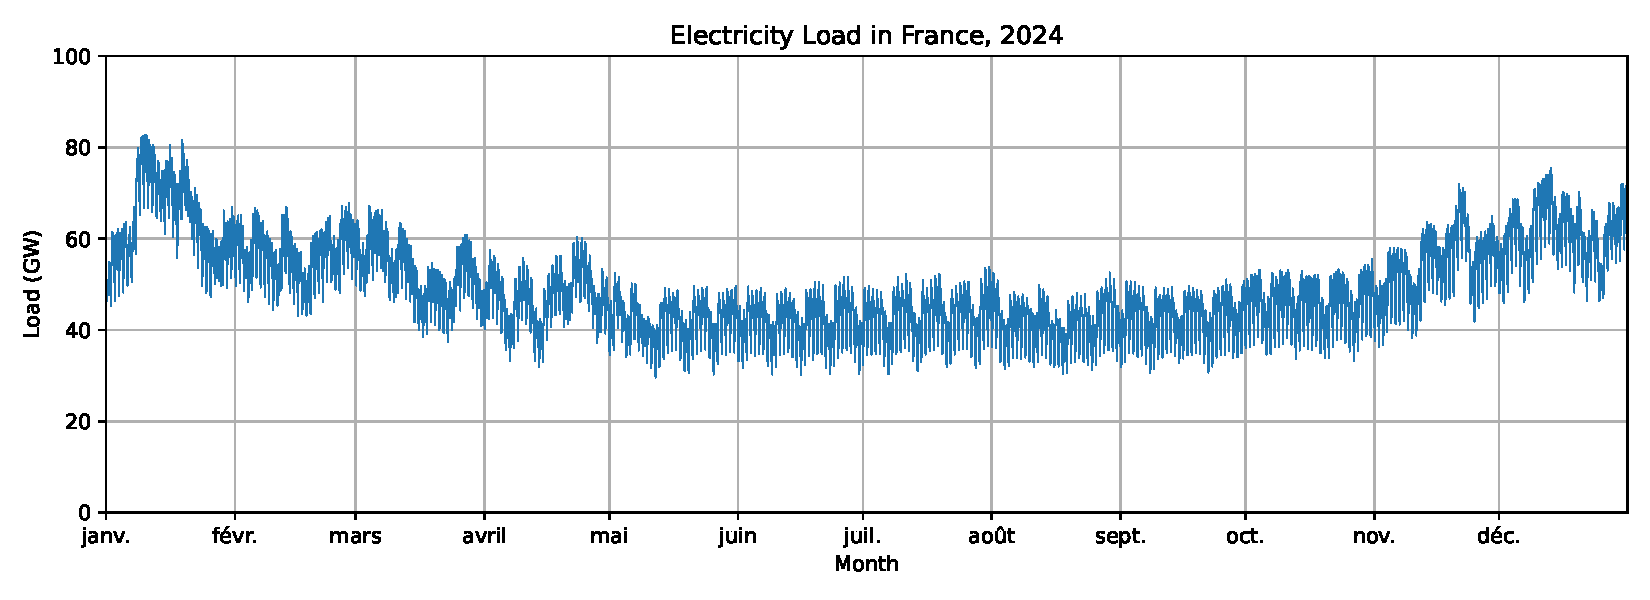
\includegraphics[width=0.95\textwidth]{figures/exercise_1-5.pdf}
  \caption{Hourly electricity load in France in 2024.}
  \label{fig:exercise1-timeseries}
\end{figure}

\subsection{Order-of-magnitude estimate of heating electricity}

The heating contribution cannot be measured directly from this file alone, since the load series does not separate end uses. A simple estimate is obtained by taking the mean load over June, July, and August as a non-heating baseline. This baseline is \SI{41.8}{\giga\watt}. Summing the positive hourly excess above this value gives
\[
E_{\mathrm{heating}} \simeq \SI{72.0}{\tera\watt\hour}.
\]
This corresponds to approximately
\[
\frac{E_{\mathrm{heating}}}{E} \simeq \SI{16.7}{\percent}
\]
of the annual electrical consumption. This result should be interpreted as an order of magnitude. It includes part of the winter-specific demand that is correlated with temperature, but it may also include other seasonal effects. Conversely, any summer cooling demand is included in the chosen baseline and is not separated.

\subsection{Load duration curve}

The load duration curve in Figure~\ref{fig:exercise1-duration} is obtained by sorting all hourly load values in decreasing order. It shows how long the power system must be able to supply a given load level. The left part corresponds to rare peak-load hours, reaching about \SI{83}{\giga\watt}. The central part is flatter and represents the majority of normal operating hours. The right part approaches \SI{30}{\giga\watt}, corresponding to low-load periods such as nights, weekends, and mild-weather days. This curve is useful for generation fleet sizing because it separates peak capacity needs from energy supplied over many hours.

\begin{figure}[H]
  \centering
  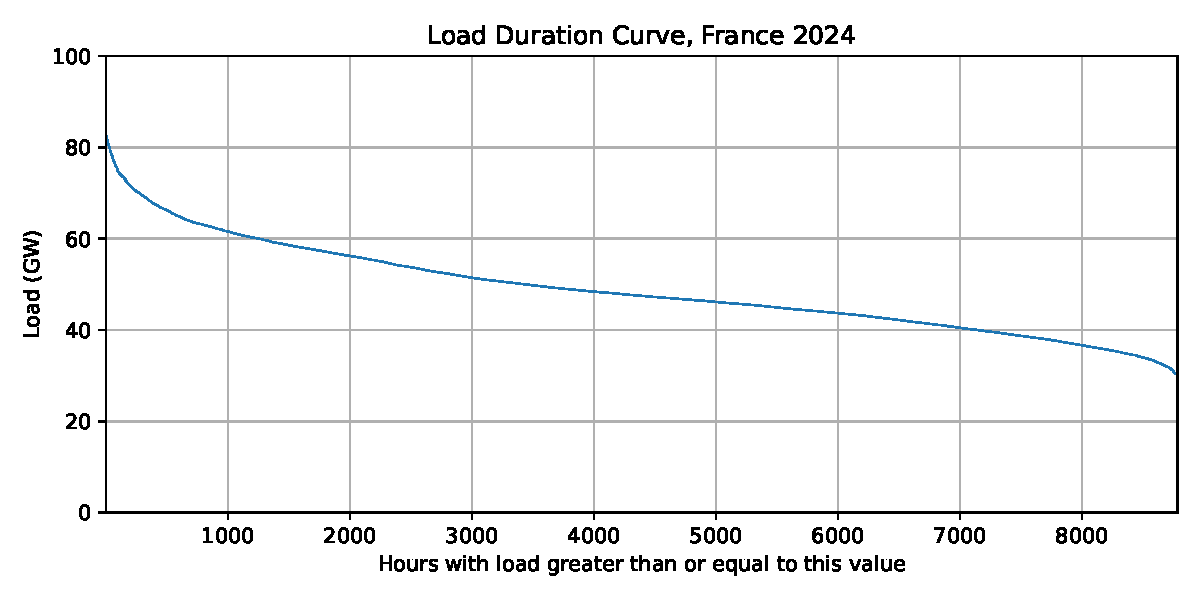
\includegraphics[width=0.82\textwidth]{figures/exercise_1-7.pdf}
  \caption{Load duration curve for the French 2024 hourly electricity load.}
  \label{fig:exercise1-duration}
\end{figure}

\subsection{Electricity demand for a fully electrified light-vehicle fleet}

For 40 million light vehicles, an annual distance of \SI{11700}{\kilo\metre} per vehicle, and a consumption of \SI{18}{\kilo\watt\hour} per \SI{100}{\kilo\metre}, the annual electricity demand is
\[
E_{\mathrm{EV}}
= 40 \times 10^6
\times 11700
\times \frac{18}{100}
= \SI{84.24e9}{\kilo\watt\hour}
= \SI{84.24}{\tera\watt\hour}.
\]
This represents about \SI{19.6}{\percent} of the 2024 electricity consumption. The value is an annual energy requirement only. The impact on peak demand would depend on charging profiles, charging power limits, and possible smart charging strategies.

\section{Exercise 2. Production analysis}

\subsection{Annual production by technology}
To be completed.

\subsection{Capacity factors}
To be completed.

\subsection{Net consumption time series}
To be completed.

\subsection{Net load duration curve}
To be completed.

\section{Exercise 3. Optimization of an adapted generation fleet}

\subsection{Annualized investment cost}
To be completed.

\subsection{Fuel and carbon costs}
To be completed.

\subsection{Production cost as a function of operating hours}
To be completed.

\subsection{Optimal generation capacities}
To be completed.

\subsection{Annual dispatch and cost assessment}
To be completed.

\section{Exercise 4. Storage sizing}

\subsection{Statistical distribution of net demand}
To be completed.

\subsection{Daily storage operation}
To be completed.

\subsection{Electric vehicle charging case}
To be completed.

\section{Optional study. Evolution of consumption}

\subsection{Renewable production scenarios}
To be completed.

\subsection{Fuel and carbon price sensitivity}
To be completed.

\subsection{Demand curve modifications}
To be completed.

\subsection{Temperature-consumption correlation}
To be completed.



%choix du style de la biblio
%\bibliographystyle{plain}
\newgeometry{
  top=0cm
}
%inclusion de la biblio
%\bibliography{references}
%voir wiki pour plus d'information sur la syntaxe des entrées d'une bibliographie

\end{document}
